\documentclass[11pt]{article}

\usepackage[margin=1in]{geometry}
\usepackage{enumitem}
\usepackage{xcolor}
\usepackage{hyperref}
\usepackage{booktabs}
\usepackage{microtype}
\usepackage{tikz}
\usepackage{tabularx}
\usepackage{longtable}
\usepackage{fancyhdr}
\usepackage{graphicx}
\usepackage{float}
\usepackage{tcolorbox}
\usepackage{amssymb}

\usetikzlibrary{shapes.geometric, arrows.meta, positioning, fit, backgrounds}

% Define colors for diagrams and callouts
\definecolor{devblue}{RGB}{66, 133, 244}
\definecolor{secgreen}{RGB}{52, 168, 83}
\definecolor{warnred}{RGB}{234, 67, 53}
\definecolor{accentyellow}{RGB}{251, 188, 4}
\definecolor{lightgray}{RGB}{245, 245, 245}

% Callout box styles
\tcbuselibrary{skins,breakable}
\newtcolorbox{keyinsight}{
  colback=secgreen!10,
  colframe=secgreen,
  fonttitle=\bfseries,
  title=Key Insight,
  breakable
}

\newtcolorbox{warning}{
  colback=warnred!10,
  colframe=warnred,
  fonttitle=\bfseries,
  title=Warning,
  breakable
}

\newtcolorbox{actionitem}{
  colback=devblue!10,
  colframe=devblue,
  fonttitle=\bfseries,
  title=Action Item,
  breakable
}

% Readability tweaks
\setlength{\parskip}{0.6em}
\setlength{\parindent}{0pt}
\linespread{1.05}

\setlist[itemize]{leftmargin=1.5em}
\setlist[enumerate]{leftmargin=1.5em}

\hypersetup{
  colorlinks=true,
  linkcolor=blue,
  urlcolor=blue
}

% Header/Footer
\pagestyle{fancy}
\fancyhf{}
\fancyhead[L]{\small Modeling AppSec Processes}
\fancyhead[R]{\small \thepage}
\renewcommand{\headrulewidth}{0.4pt}

\title{Modeling Application Security Processes with\\
\emph{Work the System}, \emph{Traction}, and \emph{This Is Service Design Doing}\\[1em]
\large A Comprehensive Guide to Building Mature, Developer-Centric Security Programs}
\author{Jordan Suber}
\date{Updated: \today}

\begin{document}

\maketitle

\begin{abstract}
This document provides a comprehensive framework for modeling Application Security (AppSec) processes by synthesizing insights from three influential books: \emph{Work the System} (Sam Carpenter), \emph{Traction} (Gino Wickman), and \emph{This Is Service Design Doing}. It offers practical guidance for transforming ad-hoc security tooling into coherent, documented systems that integrate seamlessly into modern DevSecOps workflows. The guide includes service blueprints, standard operating procedures (SOPs), metrics frameworks, maturity model alignment, and templates for immediate implementation.
\end{abstract}

\begin{center}
\textbf{Document Navigation}
\end{center}

\begin{itemize}
  \item Section~\ref{sec:purpose} -- Purpose, scope, and intended outcomes.
  \item Section~\ref{sec:books} -- How each book contributes to AppSec process modeling.
  \item Section~\ref{sec:reading-order} -- Recommended reading order for AppSec practitioners.
  \item Section~\ref{sec:modern-landscape} -- Modern AppSec tooling and threat landscape.
  \item Section~\ref{sec:pipeline-sketch} -- Service blueprints and pipeline modeling.
  \item Section~\ref{sec:sops} -- Comprehensive SOPs for key AppSec processes.
  \item Section~\ref{sec:metrics} -- Metrics framework and KPIs.
  \item Section~\ref{sec:maturity} -- Alignment with industry maturity models.
  \item Section~\ref{sec:together} -- Synthesis and implementation roadmap.
  \item Appendix~\ref{sec:templates} -- Ready-to-use templates.
  \item Appendix~\ref{sec:tooling-reference} -- Modern tooling quick reference.
\end{itemize}

\bigskip
\hrule
\tableofcontents
\bigskip
\hrule

\clearpage
\section{Purpose of This Document}
\label{sec:purpose}

\subsection{Goals}

This document serves three primary objectives:

\begin{enumerate}
  \item \textbf{Synthesize management frameworks for AppSec}: Demonstrate how three books---\emph{Work the System}, \emph{Traction}, and \emph{This Is Service Design Doing}---provide complementary perspectives for building mature security programs.
  
  \item \textbf{Provide actionable artifacts}: Deliver service blueprints, SOPs, metrics frameworks, and templates that can be adapted immediately to real-world AppSec programs.
  
  \item \textbf{Bridge tooling and process}: Move organizations from tool-centric thinking (``We use GHAS and Snyk'') to systems thinking (``We operate a coherent AppSec program with defined processes, ownership, and continuous improvement'').
\end{enumerate}

\subsection{Target Audience}

This guide is designed for:

\begin{itemize}
  \item AppSec engineers and architects seeking to formalize existing practices,
  \item Security managers building or scaling security programs,
  \item DevOps/Platform engineers integrating security into CI/CD pipelines,
  \item Engineering leadership seeking to understand and invest in AppSec maturity.
\end{itemize}

\subsection{The Transformation}

The intent is to provide an actionable path from:

\begin{quote}
  ``We have security tools and gates''\\
  \emph{to}\\
  ``We operate a coherent, documented AppSec \textbf{system} that delivers measurable security outcomes with minimal developer friction.''
\end{quote}

\begin{keyinsight}
The most effective AppSec programs treat security as an \textbf{internal service} to development teams---with clear interfaces, documented processes, measurable SLAs, and continuous improvement loops.
\end{keyinsight}

\subsection{Document Scope}

This document covers:

\begin{itemize}
  \item Secure software development lifecycle (SSDLC) processes,
  \item CI/CD security integration (SAST, SCA, secrets scanning, container security),
  \item Vulnerability management and triage,
  \item Supply chain security,
  \item Security incident response for application-layer findings,
  \item Developer enablement and security champion programs.
\end{itemize}

Out of scope: network security, infrastructure security operations, identity and access management (IAM), and compliance audit programs (though these may interface with AppSec processes).

\medskip

\textbf{Navigation tip.} If you already know these books, skim Section~\ref{sec:books} and jump to Section~\ref{sec:modern-landscape} for the modern tooling context, then proceed to the blueprints and SOPs in Sections~\ref{sec:pipeline-sketch}--\ref{sec:sops}.


\clearpage
\section{How Each Book Helps with AppSec Process Modeling}
\label{sec:books}

The three books provide complementary lenses:

\begin{center}
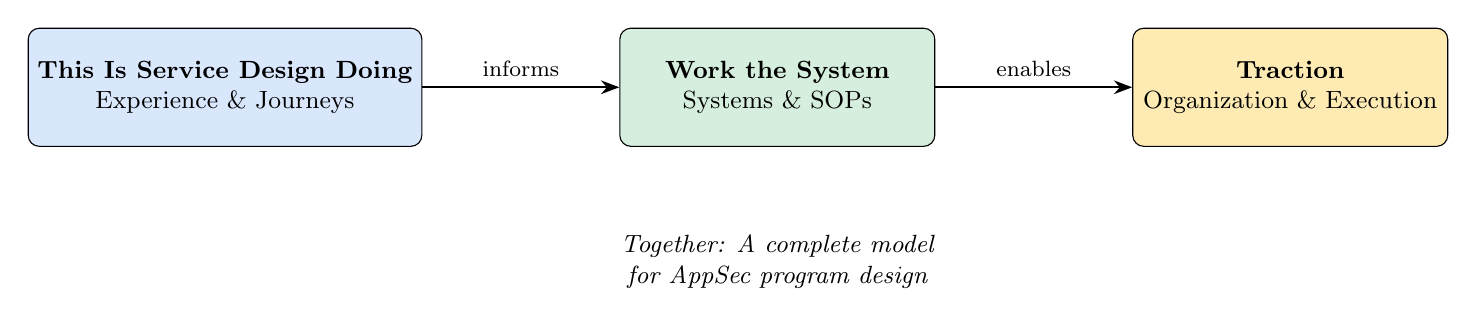
\begin{tikzpicture}[
  node distance=2.5cm,
  box/.style={rectangle, rounded corners, draw, minimum width=4cm, minimum height=1.5cm, align=center, font=\small},
]
  \node[box, fill=devblue!20] (service) {\textbf{This Is Service Design Doing}\\Experience \& Journeys};
  \node[box, fill=secgreen!20, right=of service] (wts) {\textbf{Work the System}\\Systems \& SOPs};
  \node[box, fill=accentyellow!30, right=of wts] (traction) {\textbf{Traction}\\Organization \& Execution};
  
  \draw[-{Stealth}, thick] (service) -- (wts) node[midway, above, font=\footnotesize] {informs};
  \draw[-{Stealth}, thick] (wts) -- (traction) node[midway, above, font=\footnotesize] {enables};
  
  \node[below=1cm of wts, font=\small\itshape, align=center] {Together: A complete model\\for AppSec program design};
\end{tikzpicture}
\end{center}

% --- 1. This Is Service Design Doing ---------------------------------
\subsection{\emph{This Is Service Design Doing}}
\subsubsection*{Core Idea}

\emph{This Is Service Design Doing} is a practical guide to service design that emphasizes:

\begin{itemize}
  \item Understanding users and stakeholders through research,
  \item Mapping \textbf{customer journeys} to reveal pain points and opportunities,
  \item Designing services using \textbf{service blueprints},
  \item Prototyping and iterating based on feedback.
\end{itemize}

A \textbf{service blueprint} typically includes five key swim lanes:

\begin{enumerate}
  \item \textbf{Customer actions}: What the user (developer) does,
  \item \textbf{Frontstage actions}: What the user sees and interacts with,
  \item \textbf{Backstage actions}: What the organization does behind the scenes,
  \item \textbf{Supporting processes}: Systems and integrations that enable the service,
  \item \textbf{Physical/Digital evidence}: Artifacts, communications, logs, and dashboards.
\end{enumerate}

\subsubsection*{Application to AppSec}

This book is most valuable when your goal is:

\begin{quote}
  \textbf{Design AppSec as a developer-centered service}---with clear journeys, well-defined touchpoints, responsive support, and measurable outcomes.
\end{quote}

Key applications include:

\begin{itemize}
  \item \textbf{Developer journey mapping}: Understanding how developers experience security controls throughout the SDLC---from IDE to production.
  \item \textbf{Friction identification}: Pinpointing where security processes slow down delivery or create confusion.
  \item \textbf{Touchpoint optimization}: Improving how security findings are communicated (PR annotations, dashboards, notifications).
  \item \textbf{Support channel design}: Creating clear escalation paths and self-service resources.
\end{itemize}

\begin{actionitem}
Create a developer journey map for your most common workflow (e.g., feature development with PR). Identify every point where developers interact with security tooling or policies.
\end{actionitem}

% --- 2. Work the System ----------------------------------------------
\subsection{\emph{Work the System}}
\subsubsection*{Core Idea}

\emph{Work the System} argues that every organization is a collection of \textbf{systems} and \textbf{subsystems}. To improve results consistently, you must:

\begin{itemize}
  \item Step outside the ``whirlwind'' of daily operations to see the system,
  \item Identify and isolate key systems,
  \item Document them as simple, written procedures,
  \item Improve those procedures incrementally based on real-world feedback.
\end{itemize}

The book emphasizes three foundational documents:

\begin{enumerate}
  \item \textbf{Strategic Objective}: A concise statement of what success looks like.
  \item \textbf{Operating Principles}: Decision-making guidelines that reflect organizational values.
  \item \textbf{Working Procedures}: Step-by-step documentation of how recurring work is performed.
\end{enumerate}

\subsubsection*{Application to AppSec}

Instead of viewing AppSec as a collection of tools (GHAS, Snyk, Semgrep, etc.), \emph{Work the System} encourages you to define and document the \textbf{systems} that orchestrate those tools:

\begin{itemize}
  \item \textbf{Inputs}: Events, triggers, and artifacts that initiate the process (e.g., PR opened, dependency updated, vulnerability published).
  \item \textbf{Process}: Steps, decisions, decision trees, and responsible parties.
  \item \textbf{Outputs}: Approvals, tickets, metrics, notifications, and audit records.
\end{itemize}

For AppSec, this translates to:

\begin{itemize}
  \item \textbf{Strategic Objective example}: ``We detect and remediate critical application vulnerabilities before they become exploitable in production, with minimal friction for developers and measurable improvement quarter over quarter.''
  
  \item \textbf{Operating Principles examples}:
    \begin{itemize}
      \item ``Security checks integrate into existing developer workflows---we shift left, not block.''
      \item ``We prioritize remediation by exploitability and business impact, not just severity scores.''
      \item ``Processes are documented in plain language and kept as short as practical.''
      \item ``Exceptions require documented justification and have expiration dates.''
    \end{itemize}
    
  \item \textbf{Working Procedures}: SOPs for Secure PR Flow, Vulnerability Triage, Secrets Incident Response, Dependency Management, Exception Handling, and more.
\end{itemize}

\begin{keyinsight}
The power of \emph{Work the System} is forcing explicit documentation of \textbf{who does what, when, and how}---turning tribal knowledge into repeatable, improvable systems.
\end{keyinsight}

% --- 3. Traction ------------------------------------------------------
\subsection{\emph{Traction}}
\subsubsection*{Core Idea}

\emph{Traction} introduces the Entrepreneurial Operating System (EOS), which structures organizational execution around six components:

\begin{enumerate}
  \item \textbf{Vision}: Shared understanding of organizational direction.
  \item \textbf{People}: Right people in the right seats with clear accountability.
  \item \textbf{Data}: Simple, objective metrics that drive decisions.
  \item \textbf{Issues}: Systematic identification and resolution of problems.
  \item \textbf{Process}: Documented and consistently followed systems.
  \item \textbf{Traction}: Disciplined execution through cadence and accountability.
\end{enumerate}

Key EOS tools include:

\begin{itemize}
  \item \textbf{Accountability Chart}: Who owns what (not just an org chart---role-based ownership).
  \item \textbf{Rocks}: 90-day priorities that move the needle.
  \item \textbf{Scorecard}: Weekly metrics that indicate process health.
  \item \textbf{Level 10 (L10) Meetings}: Structured weekly meetings for issue resolution.
  \item \textbf{IDS (Identify, Discuss, Solve)}: Problem-solving framework.
\end{itemize}

\subsubsection*{Application to AppSec}

\emph{Traction} provides the organizational scaffolding to ensure AppSec is not ``just a set of tools'' but a managed function with:

\begin{itemize}
  \item \textbf{Clear ownership}:
    \begin{itemize}
      \item Who owns the secure SDLC?
      \item Who owns CI/CD security gates?
      \item Who owns vulnerability management?
      \item Who owns supply chain security?
    \end{itemize}
    
  \item \textbf{Defined Rocks (90-day priorities)}:
    \begin{itemize}
      \item ``Achieve 100\% SAST coverage across production repositories.''
      \item ``Reduce critical vulnerability MTTR from 30 days to 14 days.''
      \item ``Launch security champion program with 10 trained champions.''
      \item ``Implement SBOM generation for all container images.''
    \end{itemize}
    
  \item \textbf{Scorecard metrics}:
    \begin{itemize}
      \item Open critical/high vulnerabilities by age bucket,
      \item Mean time to remediate (MTTR) by severity,
      \item Percentage of repos with security scanning enabled,
      \item Number of secrets detected in code (trend),
      \item Developer friction score (survey-based).
    \end{itemize}
    
  \item \textbf{Leadership cadence integration}:
    \begin{itemize}
      \item AppSec metrics appear on executive scorecards,
      \item AppSec issues are raised in L10 meetings,
      \item AppSec Rocks are reviewed quarterly at leadership level.
    \end{itemize}
\end{itemize}

\begin{actionitem}
Create an AppSec accountability chart mapping every key process to an explicit owner. Ensure no process is orphaned.
\end{actionitem}


\clearpage
\section{Recommended Reading Order for AppSec Modeling}
\label{sec:reading-order}

If your specific goal is to model and mature Application Security processes, a practical reading order is:

\begin{enumerate}
  \item \textbf{\emph{This Is Service Design Doing}} (Stickdorn et al.)
  
  Start here to learn tools for mapping journeys and designing services. Your first deliverable should be one or two \textbf{service blueprints} for key AppSec flows (e.g., Secure PR, Vulnerability Triage). These blueprints provide a developer-centered view of how security appears in daily work.
  
  \textit{Focus chapters}: Journey Mapping, Service Blueprinting, Prototyping.
  
  \item \textbf{\emph{Work the System}} (Sam Carpenter)
  
  Use this to transform blueprints into \textbf{SOPs}---clear, written procedures that can be followed and improved. You move from ``this is the developer journey'' to ``this is the documented system we operate.''
  
  \textit{Focus chapters}: The Systems Mindset, Strategic Objective, Working Procedures.
  
  \item \textbf{\emph{Traction}} (Gino Wickman)
  
  Finally, use EOS concepts to embed SOPs into organizational operations:
  \begin{itemize}
    \item Clarify ownership via an accountability chart,
    \item Ensure AppSec KPIs appear on scorecards,
    \item Set Rocks for quarterly improvements,
    \item Establish regular cadence for process review.
  \end{itemize}
  
  \textit{Focus chapters}: The Accountability Chart, Rocks, The Scorecard, The Issues List.
\end{enumerate}

\begin{center}
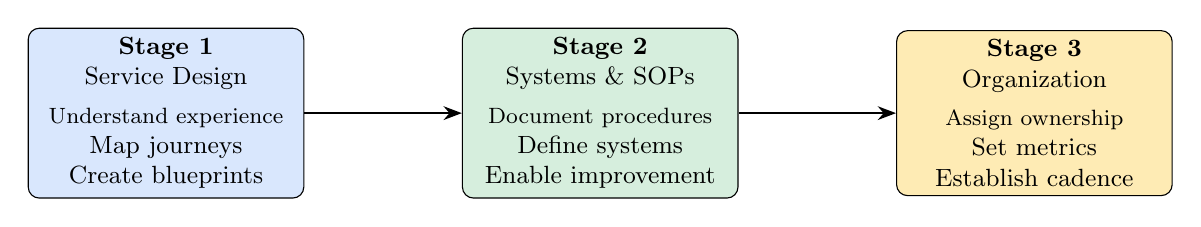
\begin{tikzpicture}[
  node distance=0.5cm and 2cm,
  stage/.style={rectangle, rounded corners, draw, minimum width=3.5cm, minimum height=2cm, align=center, font=\small},
  arrow/.style={-{Stealth}, thick}
]
  \node[stage, fill=devblue!20] (s1) {\textbf{Stage 1}\\Service Design\\[0.3em]\footnotesize Understand experience\\Map journeys\\Create blueprints};
  \node[stage, fill=secgreen!20, right=2cm of s1] (s2) {\textbf{Stage 2}\\Systems \& SOPs\\[0.3em]\footnotesize Document procedures\\Define systems\\Enable improvement};
  \node[stage, fill=accentyellow!30, right=2cm of s2] (s3) {\textbf{Stage 3}\\Organization\\[0.3em]\footnotesize Assign ownership\\Set metrics\\Establish cadence};
  
  \draw[arrow] (s1) -- (s2);
  \draw[arrow] (s2) -- (s3);
\end{tikzpicture}
\end{center}

\textbf{Navigation tip.} If you already have mature processes and want to focus on specific improvements, you can skip directly to the blueprints (Section~\ref{sec:pipeline-sketch}), SOPs (Section~\ref{sec:sops}), or metrics framework (Section~\ref{sec:metrics}).


\clearpage
\section{Modern AppSec Landscape}
\label{sec:modern-landscape}

Before diving into process modeling, it's essential to understand the current AppSec tooling landscape and threat environment. Modern AppSec has evolved significantly beyond traditional SAST/DAST.

\subsection{The Modern Threat Landscape}

Contemporary AppSec programs must address:

\begin{itemize}
  \item \textbf{Supply chain attacks}: Compromised dependencies, typosquatting, build system attacks (e.g., SolarWinds, Log4Shell, XZ Utils).
  \item \textbf{Container and cloud-native risks}: Misconfigured containers, vulnerable base images, Kubernetes security.
  \item \textbf{Infrastructure as Code (IaC) vulnerabilities}: Misconfigured Terraform, CloudFormation, or Kubernetes manifests.
  \item \textbf{API security}: Broken authentication, authorization flaws, data exposure via APIs.
  \item \textbf{AI/ML security}: Prompt injection, model poisoning, insecure AI integrations, AI-generated code risks.
  \item \textbf{Secrets exposure}: Hardcoded credentials, leaked API keys, insufficient rotation.
\end{itemize}

\subsection{Modern Tooling Categories}

\begin{table}[H]
\centering
\small
\begin{tabularx}{\textwidth}{lXl}
\toprule
\textbf{Category} & \textbf{Purpose} & \textbf{Example Tools} \\
\midrule
SAST & Static code analysis for vulnerabilities & Semgrep, CodeQL, SonarQube, Checkmarx \\
SCA & Dependency vulnerability scanning & Snyk, Dependabot, Renovate, Trivy \\
Secrets Scanning & Detect hardcoded secrets & GitLeaks, TruffleHog, GitHub Secret Scanning \\
Container Security & Image scanning, runtime protection & Trivy, Grype, Prisma Cloud, Falco \\
IaC Scanning & Infrastructure misconfigurations & Checkov, tfsec, KICS, Terrascan \\
DAST & Dynamic application testing & OWASP ZAP, Burp Suite, Nuclei \\
API Security & API-specific testing & 42Crunch, Noname Security, Salt Security \\
SBOM & Software bill of materials & Syft, CycloneDX, SPDX \\
ASPM & Application Security Posture Management & Apiiro, Cycode, ArmorCode \\
\bottomrule
\end{tabularx}
\caption{Modern AppSec tooling categories}
\label{tab:tooling}
\end{table}

\subsection{Supply Chain Security}

Supply chain security has become a critical focus area. Key practices include:

\begin{itemize}
  \item \textbf{SBOM Generation}: Creating and maintaining Software Bills of Materials for all artifacts.
  \item \textbf{Dependency pinning}: Using lock files and hash verification.
  \item \textbf{SLSA Framework}: Implementing Supply-chain Levels for Software Artifacts.
  \item \textbf{Artifact signing}: Using Sigstore/Cosign for container image and artifact signing.
  \item \textbf{Provenance attestation}: Documenting build provenance for audit trails.
  \item \textbf{Private registries}: Controlling which packages can be consumed.
\end{itemize}

\subsection{AI/ML Security Considerations}

As AI becomes integrated into development workflows, new security considerations emerge:

\begin{itemize}
  \item \textbf{AI-generated code review}: Code from Copilot, Claude, or other assistants may contain vulnerabilities or insecure patterns.
  \item \textbf{Prompt injection}: Applications using LLMs may be vulnerable to prompt injection attacks.
  \item \textbf{Model security}: Protecting ML models from extraction, poisoning, and adversarial inputs.
  \item \textbf{Data leakage}: Ensuring sensitive data isn't exposed through AI training or inference.
\end{itemize}

\begin{warning}
AI-generated code should be treated with the same (or greater) scrutiny as human-written code. Security scanning and code review remain essential.
\end{warning}

\subsection{DevSecOps Integration Principles}

Modern AppSec integrates throughout the SDLC:

\begin{center}
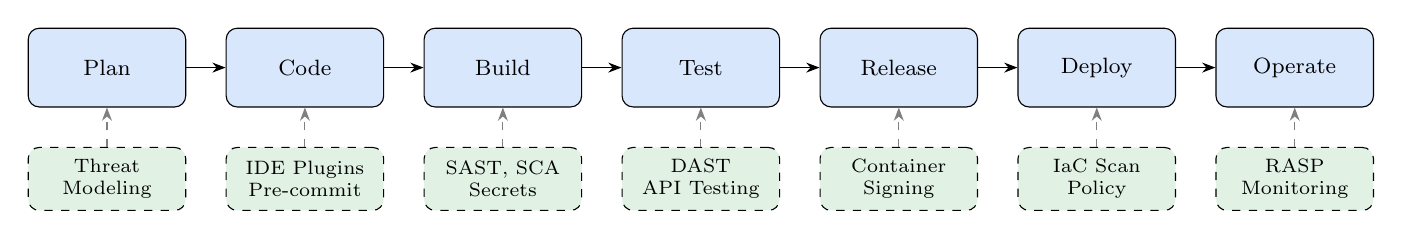
\begin{tikzpicture}[
  node distance=0.8cm,
  phase/.style={rectangle, rounded corners, draw, minimum width=2cm, minimum height=1cm, align=center, font=\footnotesize},
  security/.style={rectangle, rounded corners, draw, dashed, minimum width=2cm, minimum height=0.8cm, align=center, font=\scriptsize, fill=secgreen!15}
]
  % SDLC phases
  \node[phase, fill=devblue!20] (plan) {Plan};
  \node[phase, fill=devblue!20, right=0.5cm of plan] (code) {Code};
  \node[phase, fill=devblue!20, right=0.5cm of code] (build) {Build};
  \node[phase, fill=devblue!20, right=0.5cm of build] (test) {Test};
  \node[phase, fill=devblue!20, right=0.5cm of test] (release) {Release};
  \node[phase, fill=devblue!20, right=0.5cm of release] (deploy) {Deploy};
  \node[phase, fill=devblue!20, right=0.5cm of deploy] (operate) {Operate};
  
  % Security activities
  \node[security, below=0.5cm of plan] (s1) {Threat\\Modeling};
  \node[security, below=0.5cm of code] (s2) {IDE Plugins\\Pre-commit};
  \node[security, below=0.5cm of build] (s3) {SAST, SCA\\Secrets};
  \node[security, below=0.5cm of test] (s4) {DAST\\API Testing};
  \node[security, below=0.5cm of release] (s5) {Container\\Signing};
  \node[security, below=0.5cm of deploy] (s6) {IaC Scan\\Policy};
  \node[security, below=0.5cm of operate] (s7) {RASP\\Monitoring};
  
  % Arrows
  \foreach \i in {plan,code,build,test,release,deploy} {
    \pgfmathsetmacro{\next}{{"code","build","test","release","deploy","operate"}[
      \ifnum\pdfstrcmp{\i}{plan}=0 0\else
      \ifnum\pdfstrcmp{\i}{code}=0 1\else
      \ifnum\pdfstrcmp{\i}{build}=0 2\else
      \ifnum\pdfstrcmp{\i}{test}=0 3\else
      \ifnum\pdfstrcmp{\i}{release}=0 4\else
      5\fi\fi\fi\fi\fi
    ]}
  }
  \draw[-{Stealth}] (plan) -- (code);
  \draw[-{Stealth}] (code) -- (build);
  \draw[-{Stealth}] (build) -- (test);
  \draw[-{Stealth}] (test) -- (release);
  \draw[-{Stealth}] (release) -- (deploy);
  \draw[-{Stealth}] (deploy) -- (operate);
  
  \draw[-{Stealth}, dashed, gray] (s1) -- (plan);
  \draw[-{Stealth}, dashed, gray] (s2) -- (code);
  \draw[-{Stealth}, dashed, gray] (s3) -- (build);
  \draw[-{Stealth}, dashed, gray] (s4) -- (test);
  \draw[-{Stealth}, dashed, gray] (s5) -- (release);
  \draw[-{Stealth}, dashed, gray] (s6) -- (deploy);
  \draw[-{Stealth}, dashed, gray] (s7) -- (operate);
\end{tikzpicture}
\end{center}

Key DevSecOps principles:

\begin{itemize}
  \item \textbf{Shift left}: Detect issues as early as possible in the SDLC.
  \item \textbf{Automate everything}: Security gates should be automated, not manual.
  \item \textbf{Developer enablement}: Provide clear guidance, not just findings.
  \item \textbf{Measure and iterate}: Use data to continuously improve processes.
  \item \textbf{Blameless culture}: Focus on fixing systems, not blaming people.
\end{itemize}


\clearpage
\section{Modeling the AppSec Pipeline: Service Blueprints}
\label{sec:pipeline-sketch}

This section provides service blueprints for key AppSec processes using the \emph{This Is Service Design Doing} framework.

\subsection{High-Level AppSec Pipeline Overview}

At a high level, a modern AppSec pipeline includes:

\begin{enumerate}
  \item Developer writes code (possibly with AI assistance) and opens a PR,
  \item CI pipeline executes security scans (SAST, SCA, secrets, IaC, container),
  \item Results surface on the PR and dashboards,
  \item Developer addresses findings or requests exceptions,
  \item Approved changes merge and deploy through progressive gates,
  \item Critical findings feed into vulnerability management,
  \item Continuous monitoring operates in production.
\end{enumerate}

\subsection{Blueprint 1: Secure Pull Request Flow}

\subsubsection*{Customer (Developer) Actions}

\begin{enumerate}
  \item Create feature branch from main/trunk,
  \item Implement changes (code, tests, configuration),
  \item Run local security checks (IDE plugins, pre-commit hooks),
  \item Commit and push to remote,
  \item Open Pull Request against target branch,
  \item Review security findings annotated on PR,
  \item Address findings (fix, suppress with justification, or request exception),
  \item Respond to code review feedback,
  \item Merge when all checks pass and approvals obtained.
\end{enumerate}

\subsubsection*{Frontstage (Visible to Developer) Actions}

\begin{itemize}
  \item CI/CD pipeline status checks on PR,
  \item Inline annotations from SAST/SCA tools,
  \item Security summary comment on PR,
  \item Links to documentation/remediation guidance,
  \item Dashboard views (security overview, vulnerability trends),
  \item Exception request workflow UI.
\end{itemize}

\subsubsection*{Backstage Actions}

\begin{itemize}
  \item CI jobs orchestrating security scans,
  \item SAST engines analyzing code changes,
  \item SCA scanning dependency manifests and lock files,
  \item Secrets scanning checking for credential exposure,
  \item Container scanning for modified Dockerfiles,
  \item IaC scanning for infrastructure changes,
  \item Result aggregation and deduplication,
  \item Notification dispatch (Slack, email, ticketing).
\end{itemize}

\subsubsection*{Supporting Processes and Systems}

\begin{itemize}
  \item CI/CD platform (GitHub Actions, GitLab CI, Jenkins),
  \item Security scanning tools (configured with custom rules),
  \item Repository settings (branch protection, required checks),
  \item Secrets management platform,
  \item Ticketing system integration (Jira, Linear),
  \item Documentation platform (Confluence, Notion).
\end{itemize}

\subsubsection*{Evidence and Artifacts}

\begin{itemize}
  \item PR history and audit trail,
  \item CI/CD logs with scan results,
  \item Security finding records (with timestamps, status),
  \item Exception records with justifications,
  \item Approval audit trail,
  \item SBOM for merged changes.
\end{itemize}

\subsection{Blueprint 2: Vulnerability Triage and Management}

\subsubsection*{Customer Actions (AppSec Analyst/Developer)}

\begin{enumerate}
  \item Receive notification of new vulnerability (from scanner or external advisory),
  \item Review vulnerability details (CVSS, exploitability, affected systems),
  \item Assess business context (data sensitivity, exposure, blast radius),
  \item Assign severity and priority,
  \item Route to appropriate team/owner,
  \item Track remediation progress,
  \item Verify fix and close finding.
\end{enumerate}

\subsubsection*{Frontstage Actions}

\begin{itemize}
  \item Vulnerability dashboard with triage queue,
  \item Severity/priority assignment interface,
  \item Assignment and routing workflow,
  \item Status tracking and SLA indicators,
  \item Reporting and trends visualization.
\end{itemize}

\subsubsection*{Backstage Actions}

\begin{itemize}
  \item Vulnerability ingestion from multiple sources,
  \item Deduplication and correlation,
  \item Auto-enrichment with threat intelligence,
  \item SLA calculation and escalation triggers,
  \item Integration with ticketing systems,
  \item Metrics aggregation for reporting.
\end{itemize}

\subsubsection*{Supporting Processes}

\begin{itemize}
  \item Vulnerability database/platform,
  \item Threat intelligence feeds,
  \item Asset inventory (which repos/services exist),
  \item SLA definitions by severity,
  \item Escalation policies.
\end{itemize}

\subsubsection*{Evidence}

\begin{itemize}
  \item Triage records with justifications,
  \item Assignment and handoff history,
  \item Remediation timeline documentation,
  \item Verification evidence (scan results, test results),
  \item Exception/risk acceptance records.
\end{itemize}

\subsection{Blueprint 3: Container Security}

\subsubsection*{Customer (Developer) Actions}

\begin{enumerate}
  \item Create or modify Dockerfile/container configuration,
  \item Build container image locally or in CI,
  \item Review container scan results,
  \item Address vulnerabilities (update base image, remove packages),
  \item Push signed image to registry,
  \item Deploy using approved image.
\end{enumerate}

\subsubsection*{Frontstage Actions}

\begin{itemize}
  \item Container scan results in CI output,
  \item Registry UI showing image vulnerability status,
  \item Approved base image catalog,
  \item Deployment policy status.
\end{itemize}

\subsubsection*{Backstage Actions}

\begin{itemize}
  \item Image scanning in CI pipeline,
  \item Continuous registry scanning,
  \item Base image vulnerability monitoring,
  \item Image signing with Cosign/Sigstore,
  \item Admission controller policy enforcement,
  \item SBOM generation and storage.
\end{itemize}

\subsubsection*{Supporting Processes}

\begin{itemize}
  \item Container registry (with vulnerability scanning),
  \item Approved base image library,
  \item Kubernetes admission controller,
  \item SBOM storage and query system.
\end{itemize}

\subsubsection*{Evidence}

\begin{itemize}
  \item Image scan reports,
  \item Signing attestations,
  \item SBOM records,
  \item Deployment audit logs.
\end{itemize}

\subsection{Blueprint 4: Secrets Incident Response}

\subsubsection*{Trigger}

Secret detected in code, logs, or external exposure (e.g., GitHub public exposure alert).

\subsubsection*{Customer (Responder) Actions}

\begin{enumerate}
  \item Receive alert of exposed secret,
  \item Assess scope (what systems have access, what data is at risk),
  \item Revoke/rotate the compromised credential immediately,
  \item Audit access logs for unauthorized use,
  \item Identify root cause (how did secret get exposed),
  \item Implement preventive measures,
  \item Document incident and close.
\end{enumerate}

\subsubsection*{Frontstage Actions}

\begin{itemize}
  \item Incident alert with severity and affected secret type,
  \item Runbook links for specific secret types,
  \item Status tracking dashboard,
  \item Communication templates.
\end{itemize}

\subsubsection*{Backstage Actions}

\begin{itemize}
  \item Secret detection and alerting,
  \item Automatic ticket creation,
  \item Integration with secrets management for rotation,
  \item Log aggregation for audit,
  \item Paging/escalation if SLA breached.
\end{itemize}

\subsubsection*{Evidence}

\begin{itemize}
  \item Incident record with timeline,
  \item Rotation confirmation,
  \item Access audit results,
  \item Root cause analysis,
  \item Remediation verification.
\end{itemize}


\clearpage
\section{Standard Operating Procedures (SOPs)}
\label{sec:sops}

This section provides \emph{Work the System}-style SOPs for key AppSec processes. Each SOP follows a consistent structure: Purpose, Scope, Owner, Procedure, Exception Handling, Evidence, and Improvement Loop.

\subsection{SOP: Secure Pull Request Flow}

\paragraph{Purpose}
Ensure all code changes merged to protected branches have passed appropriate security checks and that exceptions are handled consistently with documented justification.

\paragraph{Scope}
All repositories using the standard CI/CD pipeline with security scanning enabled.

\paragraph{Owner}
AppSec Lead (process owner); Platform Engineering (tooling owner).

\paragraph{Procedure (Standard Flow)}

\begin{enumerate}
  \item Developer creates feature branch from the target branch.
  \item Developer implements changes, including appropriate tests.
  \item Developer runs local security checks (IDE plugins, pre-commit hooks) before pushing.
  \item Developer opens Pull Request to the target branch.
  \item CI pipeline triggers automatically and executes:
    \begin{itemize}
      \item Unit/integration tests,
      \item SAST scan (e.g., Semgrep, CodeQL),
      \item SCA scan (e.g., Dependabot, Snyk),
      \item Secrets scan,
      \item Container scan (if Dockerfile modified),
      \item IaC scan (if infrastructure files modified).
    \end{itemize}
  \item Results annotate the PR with findings and severity.
  \item If all required checks pass with no blocking findings:
    \begin{itemize}
      \item Developer obtains required code review approvals,
      \item PR is eligible for merge.
    \end{itemize}
  \item If blocking findings exist, proceed to Exception Handling.
\end{enumerate}

\paragraph{Exception Handling}

\begin{enumerate}
  \item Developer investigates finding and attempts remediation.
  \item If remediation is not feasible within acceptable timeframe:
    \begin{itemize}
      \item Developer creates exception request with: finding details, business justification, risk assessment, proposed mitigation, and timeline for proper fix.
    \end{itemize}
  \item Exception request is reviewed by AppSec (and security champion if applicable).
  \item AppSec either:
    \begin{itemize}
      \item Approves with conditions (maximum duration, required mitigations),
      \item Rejects with guidance for remediation.
    \end{itemize}
  \item Approved exceptions are logged with expiration date and tracked to resolution.
\end{enumerate}

\paragraph{Evidence and Records}

\begin{itemize}
  \item Scan results attached to PR,
  \item CI/CD logs,
  \item Exception request records with approval/rejection and justification,
  \item Audit trail of merges and approvals.
\end{itemize}

\paragraph{Improvement Loop}

\begin{itemize}
  \item Monthly: Review aggregate scan data, identify false positive patterns, tune rules.
  \item Quarterly: Review exception trends, identify systemic issues, update SOP as needed.
  \item Annually: Full process review with developer feedback.
\end{itemize}


\subsection{SOP: Vulnerability Triage}

\paragraph{Purpose}
Ensure newly identified vulnerabilities are assessed, prioritized, and routed for remediation consistently based on risk.

\paragraph{Scope}
All vulnerabilities from automated scanners, penetration tests, bug bounty, and external advisories.

\paragraph{Owner}
AppSec Lead (process); Vulnerability Management Analyst (execution).

\paragraph{Procedure}

\begin{enumerate}
  \item New vulnerability enters triage queue (from scanner, advisory, or manual report).
  \item Analyst reviews within SLA (Critical: 4 hours, High: 1 business day, Medium/Low: 3 business days).
  \item Analyst assesses:
    \begin{itemize}
      \item Technical severity (CVSS base score),
      \item Exploitability (is exploit available? is it being exploited in the wild?),
      \item Business context (data sensitivity, internet exposure, blast radius),
      \item Existing mitigations (WAF rules, network controls).
    \end{itemize}
  \item Analyst assigns adjusted priority:
    \begin{itemize}
      \item P1/Critical: Immediate action required, SLA 24--72 hours.
      \item P2/High: Urgent, SLA 7--14 days.
      \item P3/Medium: Standard, SLA 30--60 days.
      \item P4/Low: Backlog, address opportunistically.
    \end{itemize}
  \item Analyst routes to responsible team via ticketing system.
  \item Analyst sets SLA deadline and escalation triggers.
  \item Responsible team remediates and marks complete.
  \item Analyst verifies fix (re-scan or manual verification) and closes finding.
\end{enumerate}

\paragraph{Exception/Risk Acceptance}

\begin{enumerate}
  \item If team cannot meet SLA, they request risk acceptance.
  \item Risk acceptance requires: business justification, compensating controls, owner signature (director+ for P1/P2).
  \item Risk acceptances expire and must be renewed or resolved.
\end{enumerate}

\paragraph{Evidence}

\begin{itemize}
  \item Triage record with assessment rationale,
  \item Assignment and routing history,
  \item Remediation evidence,
  \item Risk acceptance documentation.
\end{itemize}

\paragraph{Improvement Loop}

\begin{itemize}
  \item Weekly: Review SLA compliance and escalations.
  \item Monthly: Analyze root causes of recurring vulnerability types.
  \item Quarterly: Review risk acceptance backlog, refine prioritization criteria.
\end{itemize}


\subsection{SOP: Secrets Incident Response}

\paragraph{Purpose}
Ensure exposed secrets are revoked rapidly and the incident is fully investigated to prevent recurrence.

\paragraph{Scope}
All detected secret exposures in code, logs, configuration, or external reports.

\paragraph{Owner}
AppSec Lead (process); On-call security engineer (execution).

\paragraph{Procedure}

\begin{enumerate}
  \item Alert received (automated detection or external report).
  \item Responder acknowledges within 15 minutes for production secrets.
  \item Responder assesses scope:
    \begin{itemize}
      \item What type of secret (API key, database credential, signing key)?
      \item What systems/data could be accessed?
      \item Was the exposure public or internal-only?
      \item How long was it exposed?
    \end{itemize}
  \item Responder immediately revokes/rotates the credential:
    \begin{itemize}
      \item Coordinate with service owner if rotation causes outage.
      \item If rotation not immediately possible, implement compensating controls.
    \end{itemize}
  \item Responder audits access logs for unauthorized usage.
  \item If unauthorized access confirmed, escalate to full incident response.
  \item Responder identifies root cause:
    \begin{itemize}
      \item How did the secret get committed/exposed?
      \item Why didn't existing controls catch it?
    \end{itemize}
  \item Responder implements preventive measures:
    \begin{itemize}
      \item Update .gitignore or pre-commit hooks,
      \item Improve secret scanning rules,
      \item Developer education if needed.
    \end{itemize}
  \item Responder documents incident and closes with lessons learned.
\end{enumerate}

\paragraph{Evidence}

\begin{itemize}
  \item Incident ticket with timeline,
  \item Rotation confirmation,
  \item Access audit results,
  \item Root cause analysis,
  \item Preventive measures implemented.
\end{itemize}

\paragraph{SLAs}

\begin{itemize}
  \item Production secrets (public exposure): Rotate within 1 hour.
  \item Production secrets (internal exposure): Rotate within 4 hours.
  \item Non-production secrets: Rotate within 24 hours.
\end{itemize}


\subsection{SOP: Third-Party Dependency Approval}

\paragraph{Purpose}
Ensure new dependencies are evaluated for security risk before adoption.

\paragraph{Scope}
New dependencies not previously approved, or major version upgrades with significant changes.

\paragraph{Owner}
AppSec Lead (approval authority); Developers (requesters).

\paragraph{Procedure}

\begin{enumerate}
  \item Developer identifies need for new dependency.
  \item Developer checks approved dependency list; if already approved, proceed with usage.
  \item If not approved, developer submits dependency review request:
    \begin{itemize}
      \item Package name, version, registry (npm, PyPI, etc.),
      \item Business justification,
      \item Alternatives considered.
    \end{itemize}
  \item AppSec reviews within 3 business days:
    \begin{itemize}
      \item Maintenance status (last update, maintainer activity),
      \item Known vulnerabilities,
      \item License compatibility,
      \item Dependency tree analysis,
      \item Security posture (does it follow secure development practices?).
    \end{itemize}
  \item AppSec decision:
    \begin{itemize}
      \item Approved: Added to approved list,
      \item Approved with conditions: Usage restrictions documented,
      \item Rejected: Alternative recommended.
    \end{itemize}
  \item Approved dependencies monitored for new vulnerabilities.
\end{enumerate}

\paragraph{Evidence}

\begin{itemize}
  \item Review request and decision record,
  \item Approved dependency inventory,
  \item Condition/restriction documentation.
\end{itemize}


\clearpage
\section{Metrics Framework}
\label{sec:metrics}

Effective AppSec programs require metrics that drive behavior and demonstrate value. This section provides a framework aligned with \emph{Traction}'s scorecard concept.

\subsection{Metric Categories}

\begin{table}[H]
\centering
\small
\begin{tabularx}{\textwidth}{lXl}
\toprule
\textbf{Category} & \textbf{Purpose} & \textbf{Example Metrics} \\
\midrule
\textbf{Coverage} & Are security controls deployed? & \% repos with SAST, \% images scanned \\
\textbf{Effectiveness} & Are controls finding issues? & True positive rate, findings per scan \\
\textbf{Remediation} & Are issues being fixed? & MTTR by severity, SLA compliance \\
\textbf{Risk Posture} & What is current exposure? & Open criticals, vulnerability age distribution \\
\textbf{Developer Experience} & Is security enabling or blocking? & Friction score, false positive rate \\
\textbf{Program Health} & Is the program maturing? & SOP adherence, training completion \\
\bottomrule
\end{tabularx}
\caption{AppSec metric categories}
\end{table}

\subsection{Recommended Scorecard Metrics}

For weekly/monthly leadership scorecard:

\begin{enumerate}
  \item \textbf{Open Critical Vulnerabilities}: Count of unresolved P1/Critical findings. Target: 0.
  \item \textbf{Critical MTTR}: Mean time to remediate critical findings. Target: $<$ 72 hours.
  \item \textbf{High MTTR}: Mean time to remediate high findings. Target: $<$ 14 days.
  \item \textbf{SLA Compliance Rate}: Percentage of findings resolved within SLA. Target: $>$ 95\%.
  \item \textbf{Scanning Coverage}: Percentage of production repos with security scanning enabled. Target: 100\%.
  \item \textbf{Security Gate Pass Rate}: Percentage of PRs passing security checks on first attempt. Target: $>$ 90\%.
  \item \textbf{Exception Backlog}: Count of active security exceptions. Target: Declining trend.
  \item \textbf{False Positive Rate}: Percentage of findings marked as false positive. Target: $<$ 10\%.
\end{enumerate}

\subsection{Leading vs. Lagging Indicators}

\begin{itemize}
  \item \textbf{Leading indicators} predict future security posture:
    \begin{itemize}
      \item Security training completion rate,
      \item Scanning coverage expansion,
      \item Security champion engagement,
      \item Pre-commit hook adoption.
    \end{itemize}
  \item \textbf{Lagging indicators} measure past performance:
    \begin{itemize}
      \item Vulnerabilities discovered in production,
      \item Security incidents,
      \item MTTR metrics,
      \item Audit findings.
    \end{itemize}
\end{itemize}

A healthy program tracks both.

\subsection{Metric Anti-Patterns}

Avoid metrics that drive wrong behavior:

\begin{itemize}
  \item \textbf{Raw finding counts}: Incentivizes suppressing findings rather than fixing them.
  \item \textbf{Vulnerabilities found}: Rewards noisy tools over accurate ones.
  \item \textbf{Tickets closed}: Encourages closing without proper verification.
\end{itemize}

\begin{keyinsight}
Good metrics align incentives with outcomes. Measure what matters (risk reduction, developer productivity) not what's easy to count (tickets, findings).
\end{keyinsight}


\clearpage
\section{Alignment with Industry Maturity Models}
\label{sec:maturity}

Your AppSec process modeling efforts should align with industry-recognized maturity models. This provides external validation and a roadmap for improvement.

\subsection{OWASP SAMM}

The OWASP Software Assurance Maturity Model (SAMM) provides a framework for assessing and improving software security programs across five business functions:

\begin{enumerate}
  \item \textbf{Governance}: Strategy, policy, compliance, education.
  \item \textbf{Design}: Threat assessment, security requirements, security architecture.
  \item \textbf{Implementation}: Secure build, secure deployment, defect management.
  \item \textbf{Verification}: Architecture assessment, requirements-driven testing, security testing.
  \item \textbf{Operations}: Incident management, environment management, operational management.
\end{enumerate}

Each function has three maturity levels. Your SOPs and blueprints map directly to SAMM practices.

\subsection{BSIMM}

The Building Security In Maturity Model (BSIMM) is descriptive rather than prescriptive---it measures what organizations actually do. Key domains include:

\begin{itemize}
  \item Governance,
  \item Intelligence (attack models, security features, standards),
  \item SSDL Touchpoints (architecture analysis, code review, security testing),
  \item Deployment (penetration testing, environment, operations).
\end{itemize}

BSIMM assessments benchmark your program against peers.

\subsection{NIST Cybersecurity Framework}

The NIST CSF provides high-level functions applicable to AppSec:

\begin{itemize}
  \item \textbf{Identify}: Asset inventory, risk assessment.
  \item \textbf{Protect}: Secure development, access control.
  \item \textbf{Detect}: Scanning, monitoring.
  \item \textbf{Respond}: Incident response, communications.
  \item \textbf{Recover}: Recovery planning, improvements.
\end{itemize}

\subsection{Mapping Your Program}

\begin{table}[H]
\centering
\small
\begin{tabularx}{\textwidth}{lXX}
\toprule
\textbf{Your Artifact} & \textbf{SAMM Mapping} & \textbf{NIST CSF Mapping} \\
\midrule
Secure PR SOP & Implementation: Secure Build & Protect: PR.DS \\
Vulnerability Triage SOP & Implementation: Defect Management & Detect, Respond \\
Secrets Incident SOP & Operations: Incident Management & Respond, Recover \\
Metrics Framework & Governance: Strategy \& Metrics & Identify \\
Security Champion Program & Governance: Education & Protect \\
\bottomrule
\end{tabularx}
\caption{Mapping artifacts to maturity models}
\end{table}


\clearpage
\section{Putting It All Together: Implementation Roadmap}
\label{sec:together}

This section synthesizes the frameworks, blueprints, and SOPs into a practical implementation roadmap.

\subsection{Phase 1: Foundation (Weeks 1--4)}

\begin{enumerate}
  \item \textbf{Assess current state}:
    \begin{itemize}
      \item Inventory existing security tools and their coverage,
      \item Map current (often undocumented) processes,
      \item Identify key pain points from developer feedback.
    \end{itemize}
  \item \textbf{Create developer journey map}:
    \begin{itemize}
      \item Document how developers experience security today,
      \item Identify friction points and gaps.
    \end{itemize}
  \item \textbf{Draft Strategic Objective and Operating Principles}:
    \begin{itemize}
      \item What does ``good'' look like for your AppSec program?
      \item What principles guide decisions?
    \end{itemize}
\end{enumerate}

\subsection{Phase 2: Documentation (Weeks 5--8)}

\begin{enumerate}
  \item \textbf{Create 2--3 service blueprints} for highest-impact flows:
    \begin{itemize}
      \item Secure PR Flow (almost always the starting point),
      \item Vulnerability Triage,
      \item One other based on your context (Container Security, Secrets Management).
    \end{itemize}
  \item \textbf{Write corresponding SOPs}:
    \begin{itemize}
      \item Follow the structure in Section~\ref{sec:sops},
      \item Validate with practitioners---does this match reality?
    \end{itemize}
  \item \textbf{Define initial metrics}:
    \begin{itemize}
      \item Start with 3--5 metrics from Section~\ref{sec:metrics},
      \item Establish baselines.
    \end{itemize}
\end{enumerate}

\subsection{Phase 3: Organizational Integration (Weeks 9--12)}

\begin{enumerate}
  \item \textbf{Create accountability chart}:
    \begin{itemize}
      \item Assign explicit owners to each SOP and blueprint,
      \item Ensure no orphaned processes.
    \end{itemize}
  \item \textbf{Set initial Rocks} (90-day priorities):
    \begin{itemize}
      \item Pick 2--3 measurable improvements (e.g., ``Reduce MTTR for criticals by 50\%'').
    \end{itemize}
  \item \textbf{Integrate into leadership cadence}:
    \begin{itemize}
      \item Add AppSec metrics to executive scorecard,
      \item Schedule quarterly AppSec review.
    \end{itemize}
  \item \textbf{Launch security champion program} (if not existing):
    \begin{itemize}
      \item Recruit 1 champion per team,
      \item Provide training and recognition.
    \end{itemize}
\end{enumerate}

\subsection{Phase 4: Continuous Improvement (Ongoing)}

\begin{enumerate}
  \item \textbf{Monthly}: Review metrics, tune scanning rules, address false positives.
  \item \textbf{Quarterly}: Review SOPs, update based on lessons learned, refresh Rocks.
  \item \textbf{Annually}: Full maturity assessment (SAMM or BSIMM), strategic planning.
\end{enumerate}

\subsection{The Combined Model}

The three books combine to provide:

\begin{itemize}
  \item \textbf{Service view} (\emph{This Is Service Design Doing}): Developer experience, journeys, touchpoints, support channels.
  \item \textbf{Systems view} (\emph{Work the System}): Documented SOPs, defined inputs/outputs, incremental improvement.
  \item \textbf{Organizational view} (\emph{Traction}): Ownership, metrics, cadence, accountability.
\end{itemize}

\begin{center}
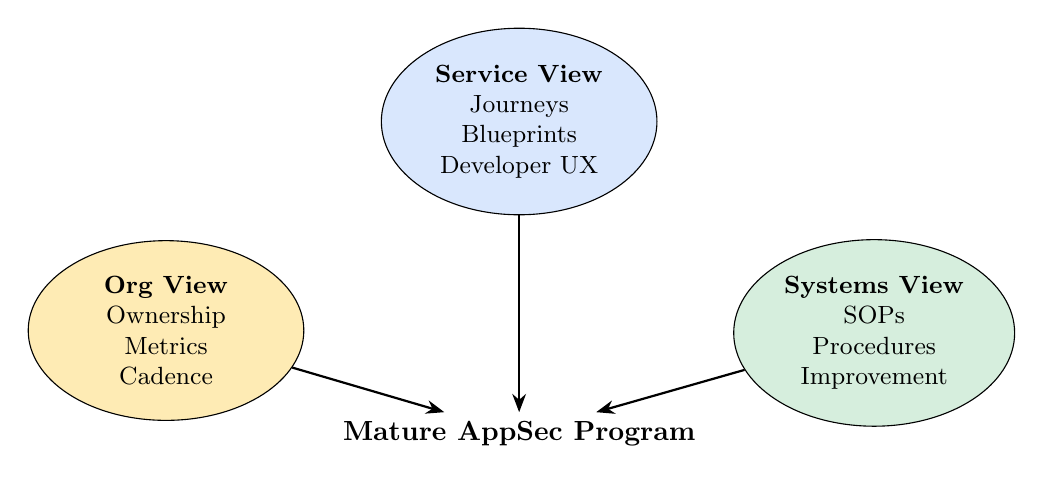
\begin{tikzpicture}[
  node distance=1.5cm,
  view/.style={ellipse, draw, minimum width=3.5cm, minimum height=2cm, align=center, font=\small}
]
  \node[view, fill=devblue!20] (service) {\textbf{Service View}\\Journeys\\Blueprints\\Developer UX};
  \node[view, fill=secgreen!20, below right=1cm and 2cm of service] (systems) {\textbf{Systems View}\\SOPs\\Procedures\\Improvement};
  \node[view, fill=accentyellow!30, below left=1cm and 2cm of service] (org) {\textbf{Org View}\\Ownership\\Metrics\\Cadence};
  
  \node[below=2.5cm of service, font=\bfseries] (center) {Mature AppSec Program};
  
  \draw[-{Stealth}, thick] (service) -- (center);
  \draw[-{Stealth}, thick] (systems) -- (center);
  \draw[-{Stealth}, thick] (org) -- (center);
\end{tikzpicture}
\end{center}

Done well, this transforms AppSec from a loose collection of tools and gates into a coherent, documented system that is easier to operate, explain, measure, and improve.


\clearpage
\appendix

\section{Templates}
\label{sec:templates}

\subsection{SOP Template}

\begin{tcolorbox}[colback=lightgray, colframe=black!50, title=SOP Template]
\textbf{SOP Title:} {[}Process Name{]}\\
\textbf{Version:} {[}X.Y{]} \quad \textbf{Last Updated:} {[}Date{]}\\
\textbf{Owner:} {[}Name/Role{]}

\medskip
\textbf{Purpose}\\{}
{[}One paragraph describing why this process exists and what outcome it ensures.{]}

\medskip
\textbf{Scope}\\{}
{[}What systems, teams, or situations does this apply to?{]}

\medskip
\textbf{Procedure}
\begin{enumerate}
  \item {[}Step 1{]}
  \item {[}Step 2{]}
  \item {[}Continue...{]}
\end{enumerate}

\medskip
\textbf{Exception Handling}\\{}
{[}How are deviations from the standard process handled?{]}

\medskip
\textbf{Evidence and Records}\\{}
{[}What artifacts document this process was followed?{]}

\medskip
\textbf{SLAs}\\{}
{[}Time-bound commitments, if applicable.{]}

\medskip
\textbf{Improvement Loop}\\{}
{[}How often is this SOP reviewed? By whom?{]}
\end{tcolorbox}

\subsection{Exception Request Template}

\begin{tcolorbox}[colback=lightgray, colframe=black!50, title=Security Exception Request]
\textbf{Requester:} {[}Name{]} \quad \textbf{Date:} {[}Date{]}\\
\textbf{Team/Service:} {[}Affected service{]}

\medskip
\textbf{Finding Details}
\begin{itemize}
  \item Finding ID: {[}Scanner finding ID{]}
  \item Severity: {[}Critical/High/Medium/Low{]}
  \item Tool: {[}Which scanner found this{]}
  \item Description: {[}Brief description{]}
\end{itemize}

\medskip
\textbf{Business Justification}\\{}
{[}Why can't this be fixed within standard SLA?{]}

\medskip
\textbf{Risk Assessment}\\{}
{[}What is the realistic risk of this vulnerability being exploited?{]}

\medskip
\textbf{Compensating Controls}\\{}
{[}What mitigations are in place to reduce risk?{]}

\medskip
\textbf{Remediation Plan}\\{}
{[}How and when will this be properly fixed?{]}\\
Proposed exception duration: {[}X days/weeks{]}

\medskip
\textbf{Approval}\\
AppSec Review: \rule{3cm}{0.4pt} Date: \rule{2cm}{0.4pt}\\
Decision: $\square$ Approved \quad $\square$ Approved with conditions \quad $\square$ Rejected
\end{tcolorbox}

\subsection{Service Blueprint Template}

\begin{tcolorbox}[colback=lightgray, colframe=black!50, title=Service Blueprint Template]
\textbf{Blueprint:} {[}Process Name{]}\\
\textbf{Version:} {[}X.Y{]} \quad \textbf{Last Updated:} {[}Date{]}

\medskip
\textbf{Customer Actions} (What the developer/user does)
\begin{itemize}
  \item {[}Action 1{]}
  \item {[}Action 2{]}
\end{itemize}

\medskip
\textbf{Frontstage Actions} (What the user sees/interacts with)
\begin{itemize}
  \item {[}Visible element 1{]}
  \item {[}Visible element 2{]}
\end{itemize}

\medskip
\textbf{Backstage Actions} (What happens behind the scenes)
\begin{itemize}
  \item {[}Backend process 1{]}
  \item {[}Backend process 2{]}
\end{itemize}

\medskip
\textbf{Supporting Processes and Systems}
\begin{itemize}
  \item {[}System 1{]}
  \item {[}System 2{]}
\end{itemize}

\medskip
\textbf{Evidence and Artifacts}
\begin{itemize}
  \item {[}Artifact 1{]}
  \item {[}Artifact 2{]}
\end{itemize}
\end{tcolorbox}


\clearpage
\section{Modern Tooling Quick Reference}
\label{sec:tooling-reference}

\begin{table}[H]
\centering
\small
\begin{tabularx}{\textwidth}{llX}
\toprule
\textbf{Tool} & \textbf{Category} & \textbf{Key Features} \\
\midrule
\multicolumn{3}{l}{\textit{Static Analysis (SAST)}} \\
Semgrep & SAST & Fast, customizable rules, supports 30+ languages \\
CodeQL & SAST & GitHub-native, semantic analysis, extensive query library \\
SonarQube & SAST & Broad language support, quality gates, enterprise features \\
\midrule
\multicolumn{3}{l}{\textit{Software Composition Analysis (SCA)}} \\
Snyk & SCA & Developer-friendly, fix suggestions, broad ecosystem \\
Dependabot & SCA & GitHub-native, automated PRs for updates \\
Renovate & SCA & Highly configurable, multi-platform \\
\midrule
\multicolumn{3}{l}{\textit{Secrets Scanning}} \\
GitLeaks & Secrets & Fast, regex and entropy detection \\
TruffleHog & Secrets & Deep history scanning, verified secrets \\
GitHub Secret Scanning & Secrets & Native integration, partner program for revocation \\
\midrule
\multicolumn{3}{l}{\textit{Container Security}} \\
Trivy & Container/SCA & Comprehensive scanner, OS and language packages \\
Grype & Container/SCA & Fast, SBOM-native \\
Prisma Cloud & Container & Enterprise, runtime protection \\
\midrule
\multicolumn{3}{l}{\textit{IaC Security}} \\
Checkov & IaC & Multi-framework, 1000+ policies \\
tfsec & IaC & Terraform-focused, fast \\
KICS & IaC & Broad IaC support, extensible \\
\midrule
\multicolumn{3}{l}{\textit{SBOM \& Supply Chain}} \\
Syft & SBOM & Generate SBOMs from containers/filesystems \\
Cosign & Signing & Container image signing, keyless support \\
SLSA & Framework & Supply chain integrity levels \\
\bottomrule
\end{tabularx}
\caption{Modern AppSec tooling reference}
\end{table}

\subsection{Tool Selection Criteria}

When evaluating tools, consider:

\begin{itemize}
  \item \textbf{Accuracy}: Low false positive rate, high true positive rate.
  \item \textbf{Developer experience}: Clear findings, actionable guidance, IDE integration.
  \item \textbf{Integration}: CI/CD compatibility, API availability, webhook support.
  \item \textbf{Customization}: Can you write custom rules for your context?
  \item \textbf{Performance}: Scan time acceptable for CI/CD?
  \item \textbf{Coverage}: Languages, frameworks, and package ecosystems you use.
  \item \textbf{Total cost}: License cost, maintenance burden, training investment.
\end{itemize}


\clearpage
\section*{Document History}

\begin{tabular}{lll}
\toprule
\textbf{Version} & \textbf{Date} & \textbf{Changes} \\
\midrule
1.0 & Initial & Original document \\
2.0 & \today & Comprehensive update: Added modern tooling landscape, \\
    &        & supply chain security, AI/ML considerations, additional \\
    &        & blueprints (Container Security, Secrets Incident Response), \\
    &        & expanded SOPs, metrics framework, maturity model alignment, \\
    &        & implementation roadmap, templates, and tooling reference. \\
\bottomrule
\end{tabular}

\end{document}